\chapter*{Programme officiel}

\section*{Programme officiel}

Les langages de programmation Turing-complets sont caractérisés par un corpus de « cons-tructions élémentaires ». Sans introduire cette terminologie, il s'agit de montrer qu'il existe de nombreux langages de programmation, différents par leur style (impératif, fonctionnel, objet, logique, événementiel, etc.), ainsi que des langages formalisés de description ou de requêtes qui ne sont pas des langages de programmation.

L'importance de la spécification, de la documentation et des tests est à présenter, ainsi que l'intérêt de la modularisation qui permet la réutilisation de programmes et la mise à disposition de bibliothèques. Pour les programmes simples écrits par les élèves, on peut se contenter d'une spécification rapide mais précise.

{\centering\begin{tabular}{|L{3cm}|L{5.5cm}|L{6cm}|}\hline
\cellcolor{bo}\bfseries\textcolor{white}{Contenus}&
\cellcolor{bo}\bfseries\textcolor{white}{Capacités attendues}&
\cellcolor{bo}\bfseries\textcolor{white}{Commentaires}\\ \hline
Constructions élémentaires
&
Mettre en évidence un corpus de constructions élémentaires.
& Séquences, affectation, conditionnelles, boucles bornées, boucles non bornées, appels de fonction.\\ \hline
Diversité et unité des langages de programmation
&
Repérer, dans un nouveau langage de programmation, les traits communs et les traits particuliers à ce langage.
&
Les manières dont un même programme simple s'écrit dans différents langages sont comparées.\\ \hline
Spécification
&
Prototyper une fonction.

Décrire les préconditions sur les arguments.

Décrire des postconditions sur les résultats.
&
Des assertions peuvent être utilisées pour garantir des préconditions ou des postconditions.\\ \hline
Mise au point de programmes
&
Utiliser des jeux de tests.
&
L'importance de la qualité et du nombre des tests est mise en évidence.

Le succès d'un jeu de tests ne garantit pas la correction d'un programme.\\ \hline
Utilisation de bibliothèques
&
Utiliser la documentation d'une bibliothèque.
&
Aucune connaissance exhaustive d'une bibliothèque particulière n'est exigible.\\ \hline
\end{tabular}\par}


\chapter{Constructions élémentaires}

Cette partie est volontairement non détaillée pour tenir sur une page de référence. Ces notions ont déjà été rencontrées en particulier en mathématiques avant l'entrée en Première.

\begin{multicols}{2}

{\bfseries Valeurs}

\begin{itemize}
	\item \pythoninline{1} est de type \pythoninline{int}
	\item \pythoninline{1.0} est de type \pythoninline{float}
	\item \pythoninline{True} est de type \pythoninline{bool}
	\item \pythoninline{'1'} est de type \pythoninline{str}
	\item \pythoninline{[1, 2]} est de type \pythoninline{list}
	\item \pythoninline{(1, 2)} est de type \pythoninline{tuple}
	\item \pythoninline{{'un' : 1, 'deux' : 2}}  de type \pythoninline{dict}
\end{itemize}

\medskip
{\bfseries Variables}

L'affectation \fbox{$x\leftarrow 1$} : \pythoninline{x = 1}.


\medskip
{\bfseries Conditionnelle}

\begin{algorithm}[H]
$x \leftarrow 96$\;
\lSi{$x$ est pair}{$x \leftarrow \frac{x}{2}$}
\end{algorithm}

\vspace{-1ex}
\begin{minted}{python}
x = 96
if x % 2 == 2 :
    x = x // 2
\end{minted}

\begin{algorithm}[H]
$x \leftarrow 96$\;
\lSi{$x$ est pair}{$x \leftarrow \frac{x}{2}$}
\lSinon{$x \leftarrow x * 3 + 1$}
\end{algorithm}

\vspace{-1ex}
\begin{minted}{python}
x = 96
if x % 2 == 2 :
    x = x // 2
else :
    x = x * 3 + 1
\end{minted}

\begin{algorithm}[H]
$x \leftarrow $ entier aléatoire entre -5 et 5\;
\lSi{$x>0$}{ $x \leftarrow x + 1$ }
\lSinonSi{$x<0$}{$x \leftarrow x - 1$}
\lSinon{$x \leftarrow 1$ ou $-1$ au hasard}
\end{algorithm}

\vspace{-1ex}
\begin{minted}{python}
from random import randint

x = randint(-5,5)
if x > 0 :
    x = x + 1
elif x < 0 :
    x = x - 1
else :
    x = 1 - 2 * randint(0,1)
\end{minted}



\medskip
{\bfseries Boucle non bornée}

\begin{algorithm}[H]
$x \leftarrow 96$\;
\Tq {$x$ est pair}
{   
    $x \leftarrow \frac{x}{2}$\;
}
\end{algorithm}

\vspace{-1ex}
\begin{minted}{python}
x = 96
while x % 2 == 0 :
    x = x // 2
\end{minted}


\medskip
{\bfseries Boucle bornée}

\begin{algorithm}[H]
\Pour{$k$ {\normalfont\bfseries allant de} $0$ {\normalfont\bfseries à} $9$}
{ affiche($k$)\; }
\end{algorithm}

\vspace{-1ex}
\begin{minted}{python}
for k in range (10) :
    print(k)
\end{minted}

\begin{itemize}
	\item \pythoninline{range(n)} de $0$ à $n-1$
	\item \pythoninline{range(d,n)} de $d$ à $n-1$
	\item \pythoninline{range(d,n,p)} de $d$ à $n-1$ de $p$ en $p$
\end{itemize}

Avec $d$, $n$ et $p$ entiers.

Peut aussi être utilisé directement sur les types \pythoninline{str}, \pythoninline{list}, \pythoninline{tuple} et \pythoninline{dict}.


\medskip
{\bfseries Fonction}


\begin{minted}{python}
def f(x) :
    x = x * 2
    return x

x = 3
y = f(x)
print('f(',x,') = ',y, sep = '')
\end{minted}

La variable \pythoninline{x} de la fonction est dite locale. Elle copie la référence obtenue par le paramètre. Changer sa valeur ne change donc pas celle de la variable \pythoninline{x} externe à la fonction.

Pour un type construit (un tableau), cette référence donne accès aux éléments qui, si modifiés, le sont alors de manière globale.

\end{multicols}

\chapter{Différents langages}

En introduction, voici quelques façons de produire dans différents langages, l'affichage des mots << Hello, world ! >>, à commencer par Python :

\vspace{-2ex}
\begin{minted}{python}
print('Hello, world!')
\end{minted}

\begin{multicols}{2}
Langage Bash :

\vspace{-2ex}
\begin{minted}{bash}
#!/bin/bash
echo 'Hello, world!'
\end{minted}

Langage C :

\vspace{-2ex}
\begin{minted}{C}
#include <stdio.h>

int main()
{
    printf("hello, world");
    return 0;
}
\end{minted}

Langage HTML5 :

\vspace{-2ex}
\begin{minted}{html}
<!DOCTYPE html>
<html>
    <head>
        <meta charset="utf-8">
        <title>Hello, world!</title>
    </head>
    <body>
        <p>Hello, world!</p>
    </body>
</html>
\end{minted}

Langage Java :

\vspace{-2ex}
\begin{minted}[fontsize = \footnotesize]{java}
public class HelloWorld {
    public static void main(String[] args) {
        System.out.println("Hello, world!"); 
    }
}
\end{minted}

Langage JavaScript :

\vspace{-2ex}
\begin{minted}{js}
console.log("Hello, world!");
\end{minted}

Langage \LaTeX (utilisé pour ce document) :

\vspace{-2ex}
\begin{minted}{latex}
\documentclass{minimal}
\begin{document}
Hello, world!
\end{document}
\end{minted}

Langage PHP :

\vspace{-2ex}
\begin{minted}{php}
<?php
 echo "Hello, world!";
?>
\end{minted}
\end{multicols}

À première vue, ils semblent très différents, mais le plus important est qu'ils peuvent tous faire une même chose : produire un affichage de texte !
\medskip

HTML et LATEX sont deux langages à balises de définition de documents. On peut identifier \mintinline{html}{<html>...</html>} et  \mintinline{html}{\begin{document}...\end{document}}. L'un destine son résultat à l'écran et l'autre à l'impression, mais ils sont très comparables.
  
\medskip

Python, C, Java, ... sont des langages de programmation impératifs. On y retrouve
\begin{itemize}
  \item des séquences d'instructions, séparées par un simple passage à la ligne pour Python, par un point-virgule \mintinline{C}{;} dans beaucoup d'autres langages ;
  
  \item des affectations, \mintinline{C}{x = 3} en Python, C, Java, JavaScript... ; \mintinline{C}{$x = 3} en PHP ; %$
  
  ( \mintinline{C}{x := 3}, \mintinline[escapeinside=||]{C}{x |$\leftarrow$| 3} ou encore  \mintinline[escapeinside=||]{C}{3 |$\rightarrow$| x} ... dans d'autres langages. )
  
  \item des instructions conditionnelles :

\begin{multicols}{2}  
  en Python :
  
  
  \vspace{-2ex}
\begin{minted}{python3}
if (x == 3) :
    print("Ok")
\end{minted}
  
  
   en JavaScript :
  
  \vspace{-2ex}
\begin{minted}{javascript}
if (x == 3) {
    console.log("Ok");
}
\end{minted}
  \end{multicols}

Dans beaucoup de langages, les blocs d'instructions  sont délimités par des accolades  \mintinline{C}{{ ... }}, quand, en Python, ils commencent après \mintinline{python3}{:} et sont identifiés par une indentation.
  
  \item des boucles :

\begin{multicols}{2}  
  boucle \texttt{pour} en Python :
  
  
  \vspace{-2ex}
\begin{minted}{python3}
chiffres = ""
for i in range(10) :
    chiffres = chiffres + i
\end{minted}
  
  
   en JavaScript :
  
  \vspace{-2ex}
\begin{minted}{javascript}
var chiffres = "";
for (var i = 0; i < 10; i++) {
  chiffres = chiffres + i;
}
\end{minted}
\end{multicols}

En JavaScript la boucle \texttt{pour} est définie par une initialisation, une condition à vérifier pour continuer et une instruction à exécuter en fin de boucle. (Une autre syntaxe, proche de celle de Python existe en JavaScript). Certains langages sont plus proches du \texttt{pour} algorithmique.


La boucle \texttt{while} est semblable pour les langages proposés ici. On remplace \mintinline{python3}{if} par \mintinline{python3}{while} pour répéter le bloc conditionnel.
  
  \item des branchements.
  
  Il s'agit de possibilités de sauter d'une partie du programme à une autre. En particulier l'appel à une fonction.
  
  

\begin{multicols}{2}  
  Fonction en Python :
  
  
  \vspace{-2ex}
\begin{minted}{python3}
def f(x) :
    return x * x 
\end{minted}
  
  
   En JavaScript :
  
  \vspace{-2ex}
\begin{minted}{javascript}
function f(x) {
  return x * x;
}
\end{minted}


  
  
   En C :
  
  \vspace{-2ex}
\begin{minted}{c}
int f(int x)
{
    return x * x;
}
\end{minted}

Et l'appel (commun à ces langages)

\pythoninline{f(7)} renvoie 49.

\end{multicols}
  
  
  
\end{itemize} 

\medskip

Il existe d'autres types de programmation qui pourront être discutés en Terminale.


\chapter{Spécification et tests}

\section{Prototype d'une fonction}

\Cours{{\bfseries Prototype} 

Le prototype d'une fonction est sa \emph{signature}. Il définit : 

\begin{itemize}
	\item le nom de la fonction,
	\item le nombre et le type de ses paramètres,
	\item le type de la valeur qu'elle renvoie.
\end{itemize}
}

Avec les langages C ou Java par exemple, on écrit le prototype des fonctions. Cela permet par exemple d'écrire la partie principale en début de code contrairement au langage Python. La commande \pythoninline{def} définit la fonction en place ; elle n'a aucune existence pour le code la précédant.

\begin{multicols}{2}  
  Fonction en Python :
  
  (Pas de prototype)
  
  \vspace{-2ex}
\begin{minted}{python3}
def f(x) :  # Définition en place
    return x * x 
\end{minted} 
  
   En C :
  
  \vspace{-2ex}
\begin{minted}{c}
int f(int x)  // Prototype
{
    return x * x;
}
\end{minted}
\end{multicols}

Un des avantages d'une fonction sans prototype est qu'elle peut éventuellement être utilisée avec des valeurs de types différents : \pythoninline{f(3.5)} sera évalué correctement en Python, mais sera refusé par le compilateur C qui attend un argument entier.

Un des inconvénients est qu'on perd en lisibilité sur l'intention de la fonction. C'est pourquoi il est important de commenter son code, en particulier chaque fonction pour préciser sa spécification.

\section{Spécification}

\Cours{{\bfseries Spécification} 

La spécification d'un algorithme (et donc d'une fonction) définit :
  
  \vspace{-2ex}
\begin{multicols}{2}
\begin{itemize}
	\item les entrées et sorties
	\item le rôle
	\item les préconditions
	\item les postconditions
\end{itemize}
\end{multicols}
}
\begin{itemize}
	\item Les entrées et sorties sont ce qui fait le prototype d'une fonction.

	\item Le rôle est une description du problème que résout l'algorithme (la fonction).

	\item Les préconditions sont des précisions sur la nature exacte des entrées.

	\item Les postconditions sont des précisions sur la nature exacte des sorties.
\end{itemize}


Les préconisations sont les hypothèses (au sens mathématique) sur les entrées, permettant de démontrer que l'algorithme (ou la fonction) joue bien son rôle, c'est à dire produit des sorties vérifiant les postconditions.

\medskip

Avec le langage Python on écrit la spécification avec le code dans des \emph{docstring}. C'est un texte entouré de guillemets triples qui se place juste en début de code :

  
  \vspace{-2ex}
\begin{minted}{python3}
def f(x):
    """Renvoie le carré du nombre donné en argument."""
    return x * x
\end{minted}

Pour un algorithme simple comme celui-ci, une seule ligne précisant son rôle peut suffire. Mais il n'est pas rare que le \emph{docstring} soit plus long que le code lui-même :

  
  \vspace{-2ex}
\begin{minted}{python3}
def centSur(x):
    """Calcule le quotient entier de 100 par x.
    
    Cette fonction opère la division entière de 100 par x et en
    renvoie le quotient.
    
    :param x: Un entier non nul.
    :type x: int
    :return: Le quotient de la division entière de 100 par x
    :rtype: int
    """
    return 100 // x
\end{minted}

Cette exemple utilise la syntaxe RST mais ce n'est pas une obligation. 
 
 On obtient alors l'affichage de cette documentation avec la commande \pythoninline{help(centSur)}.

\section{Tests et assertions}

Un \emph{docstring} permet de documenter en écrivant la spécification des fonctions. Il permet aussi la mise au point des programmes à l'aide de jeux de tests. En effet, juste après la spécification, et avant même de réfléchir à l'algorithme, on peut mettre en place un jeu de tests qu'il devrait passer pour avoir une chance de résoudre le problème posé.

\begin{minted}{python3}
def centSur(x):
    """Calcule le quotient entier de 100 par x.
    
    >>> centSur(3)
    33
    """
    return 100 // x
\end{minted}

La bibliothèque \pythoninline{doctest} permet effectivement de lancer tous les tests par la commande \pythoninline{doctest.testmod()}. Pour voir tous les tests effectués, on peut compléter cette commande  en \pythoninline{doctest.testmod(verbose = True)}.

 La réussite à ces tests n'est pas une preuve de correction, mais permet de guider la programmation et l'utilisateur.
 
 \medskip
 
 En phase de conception ou plutôt de débogage, on peut vouloir s'assurer que les préconditions sont effectivement remplies. Dans ce cas, on utilise des assertions : on exprime chacune des préconditions après le mot clef \pythoninline{assert}. 
 
\begin{minted}{python3}
def centSur(x):
    """Calcule le quotient entier de 100 par x."""
    assert isinstance(x, int)
    assert x != 0
    return 100 // x
\end{minted}

Avec ce code, par exemple, \pythoninline{centSur(5.0)} provoquera une erreur, alors que sans la première assertion, il aurait donné une réponse.

\chapter{Utilisation de bibliothèques}

\Cours{{\bfseries Bibliothèque}

Une bibliothèque, on dit souvent un \emph{module} en Python, est un fichier contenant un ensemble de fonctions, de classes (types personnalisés), et de constantes, que l'on peut importer dans son propre programme pour les utiliser.
}

\section{Utilisation de modules existants}

Il existe de très nombreux modules en Python (c'est un des avantages de ce langage). Certains sont dits \emph{standards} et fournis avec l'installation du langage. D'autres doivent être installés manuellement.

Parmi les standards, notons :

\begin{itemize}
	\item \pythoninline{random} dont la fonction \pythoninline{randint()} permet d'obtenir un entier aléatoire dans un intervalle,
	\item \pythoninline{math} qui contient par exemple \pythoninline{cos()} et \pythoninline{sin()},
	\item \pythoninline{doctest} pour implémenter des tests automatiques de fonctions,
	\item \pythoninline{csv} pour le traitement de tables CSV,
	\item \pythoninline{json} pour le traitement de données JSON,
	\item \pythoninline{socket} pour les connexions TCP/IP,
	\item \pythoninline{os} et \pythoninline{sys} pour les fonctions système.
\end{itemize}

Parmi les autres, on peut citer :

\begin{itemize}
	\item \pythoninline{PIL} pour le traitement d'images (à charger sous le nom \pythoninline{pillow}),
	\item \pythoninline{requests} pour les requêtes HTTP GET et POST,
	\item \pythoninline{http.server} pour un serveur HTTP (réponse aux GET et POST).
\end{itemize}

\medskip

Pour utiliser une bibliothèque déjà installée, on peut employer une des méthodes suivantes :

\begin{multicols}{2}
\begin{minted}{python3}
import random

x = random.randint(1,9)
\end{minted}

\begin{minted}{python3}
import random as hasard

x = hasard.randint(1,9)
\end{minted}

\begin{minted}{python3}
from random import randint

x = randint(1,9)
\end{minted}

\begin{minted}{python3}
from random import randint as hasard

x = hasard(1,9)
\end{minted}
\end{multicols}

\medskip

Pour une bibliothèque non standard, il faut passer en ligne de commande pour la charger et l'installer avec le module \pythoninline{pip}. Par exemple pour \pythoninline{PIL} :

\noindent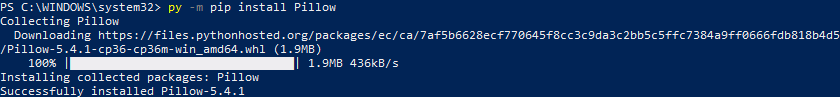
\includegraphics[width=\textwidth]{images/installPillow.png}

\section{Conception de modules}

N'importe quel fichier Python est un module dont le nom est celui du fichier. Il est donc très simple d'en concevoir un :

\begin{multicols}{2}
Fichier \texttt{Bonjour.py} :

\vspace{-2ex}
\begin{minted}{python3}
""" Ceci est le module Bonjour """

def hello():
    """ Affiche : Bonjour ! """
    print('Bonjour !')

hello()
\end{minted}

Script dans le même répertoire :

\begin{minted}{python3}
import Bonjour

Bonjour.hello()
\end{minted}

Ce second script s'exécute bien...

Mais dit bonjour deux fois !
\end{multicols}

Au moment de l'importation, le script contenu dans le module est entièrement exécuté. Comme il contient un appel à la fonction \pythoninline{hello()}, on obtient un premier affichage, puis un second dû à l'appel \pythoninline{Bonjour.hello()} du second script.

On pourrait enlever le \pythoninline{hello()} du module, mais dans la pratique, on souhaite souvent garder à un module la possibilité de s'exécuter en tant que script principal. Il suffit pour cela d'ajouter une conditionnelle :

\begin{multicols}{2}
\begin{minted}{python3}
""" Ceci est le module Bonjour """

def hello():
    """ Affiche bonjour """
    print('Bonjour !')
    
if __name__ == "__main__":
    hello()
\end{minted}

Par exemple, en phase de développement, on pourra utiliser :

\begin{minted}{python3}
if __name__ == '__main__':
   import doctest
   doctest.testmod()
\end{minted}
\end{multicols}

Si on prend l'exemple proposé pour l'explication sur les assertions, on obtient :

\begin{minted}{python3}
""" Module de test sur les assertions """

def centSur(x):
    """Calcule le quotient entier de 100 par x.
    
    Cette fonction opère la division entière de 100 par x et en
    renvoie le quotient.    
    
    :param x: Un entier non nul
    :type x: int
    :return: Le quotient de la division entière de 100 par x
    :rtype: int
    
    >>> centSur(3)
    33
    
    >>> centSur(3.0)
    Traceback (most recent call last):
        ...
    AssertionError: x doit être entier
    
    >>> centSur(0)
    Traceback (most recent call last):
        ...
    AssertionError: x ne doit pas être nul
    """
    assert isinstance(x, int), 'x doit être entier'
    assert x != 0, 'x ne doit pas être nul'
    return 100 // x

if __name__ == '__main__':
    import doctest
    doctest.testmod(verbose=True)
\end{minted}